\chapter{Chapter title goes here} \label{chap:chap-3}

% epigraph after chapter heading
\epigraph{Since it is written in \LaTeX, it must be true.}{-- Isaac Newton}

%%%% MUST: add the citation for the chapter if it is a reprint

%% remove the following and add your chapter text here
\section{Introduction}
\blindtext

\section{Current approach}
\blindtext\footnote{Hello, this is the first footnote with no
  indentation and single-spaced text. The spacing between two footnotes
is also single-spaced.}

\subsection{Hypothesis statement}
\blindtext\footnote{This is the second footnote.}

\subsection{Experimental evidences}

\begin{figure}[ht]
  \begin{center}
    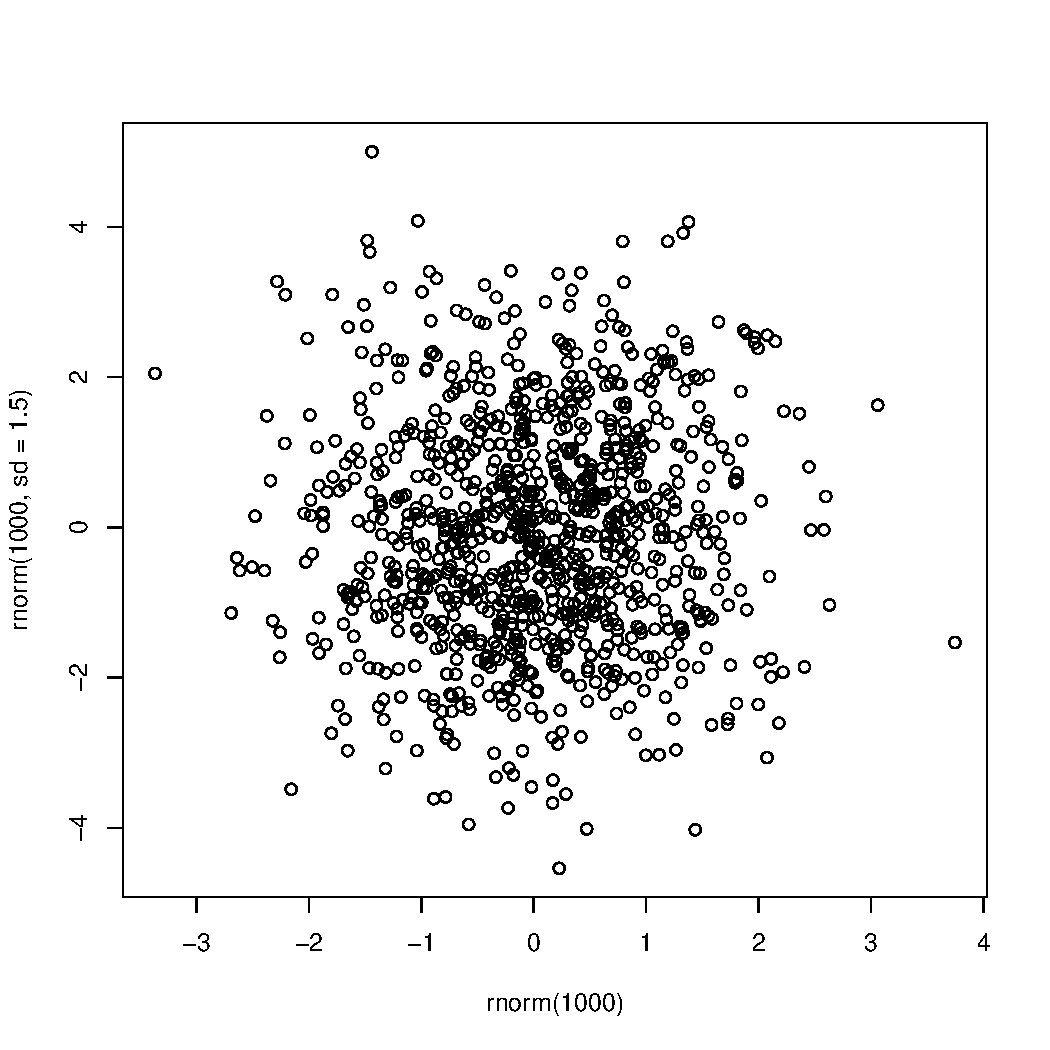
\includegraphics[width=\textwidth, trim={6cm 5cm 6cm
    5cm},clip,page=1] {chap3.pdf}
    \caption{Random dots in the chapter 3 directory.}
    \label{fig:dots}
  \end{center}
\end{figure}


\subsubsection{Data analysis}
\blindtext
